\documentclass{article}
\usepackage{amsmath}
\usepackage{mathtools}
\usepackage{ifpdf}
\usepackage{subcaption}
\usepackage{graphicx}
\usepackage{caption}

\newcommand {\arrowedbox}[1] {{\rightarrow\fbox{#1}\rightarrow}} %draw box with arrow

\begin{document}


Lorem ipsum dolor sit amet, consectetur adipiscing elit. Cras eget efficitur metus. Curabitur maximus lobortis arcu at fermentum. Pellentesque ante enim, iaculis ullamcorper ultrices non, ornare id arcu. Suspendisse hendrerit erat id turpis feugiat, in convallis libero fringilla. Vivamus non ligula id nisl egestas ultrices eu in augue. Morbi rhoncus, felis at feugiat imperdiet, mauris metus cursus nulla, id aliquet odio arcu in orci. Sed eget risus id dolor euismod convallis vel at arcu. Vestibulum ultrices massa arcu, eu tincidunt orci dictum ut. Aenean lacinia urna quam, non auctor nibh tempor vitae. Cras sagittis ex et massa commodo fermentum. Praesent commodo orci ornare odio sollicitudin, id gravida quam sagittis. Donec auctor id nisi at placerat. Proin auctor mauris ut tincidunt tempor. Pellentesque habitant morbi tristique senectus et netus et malesuada fames ac turpis egestas. 

\begin{figure}[htpb]
    \centering
    \begin{subfigure}{0.45\textwidth}
      \centering
      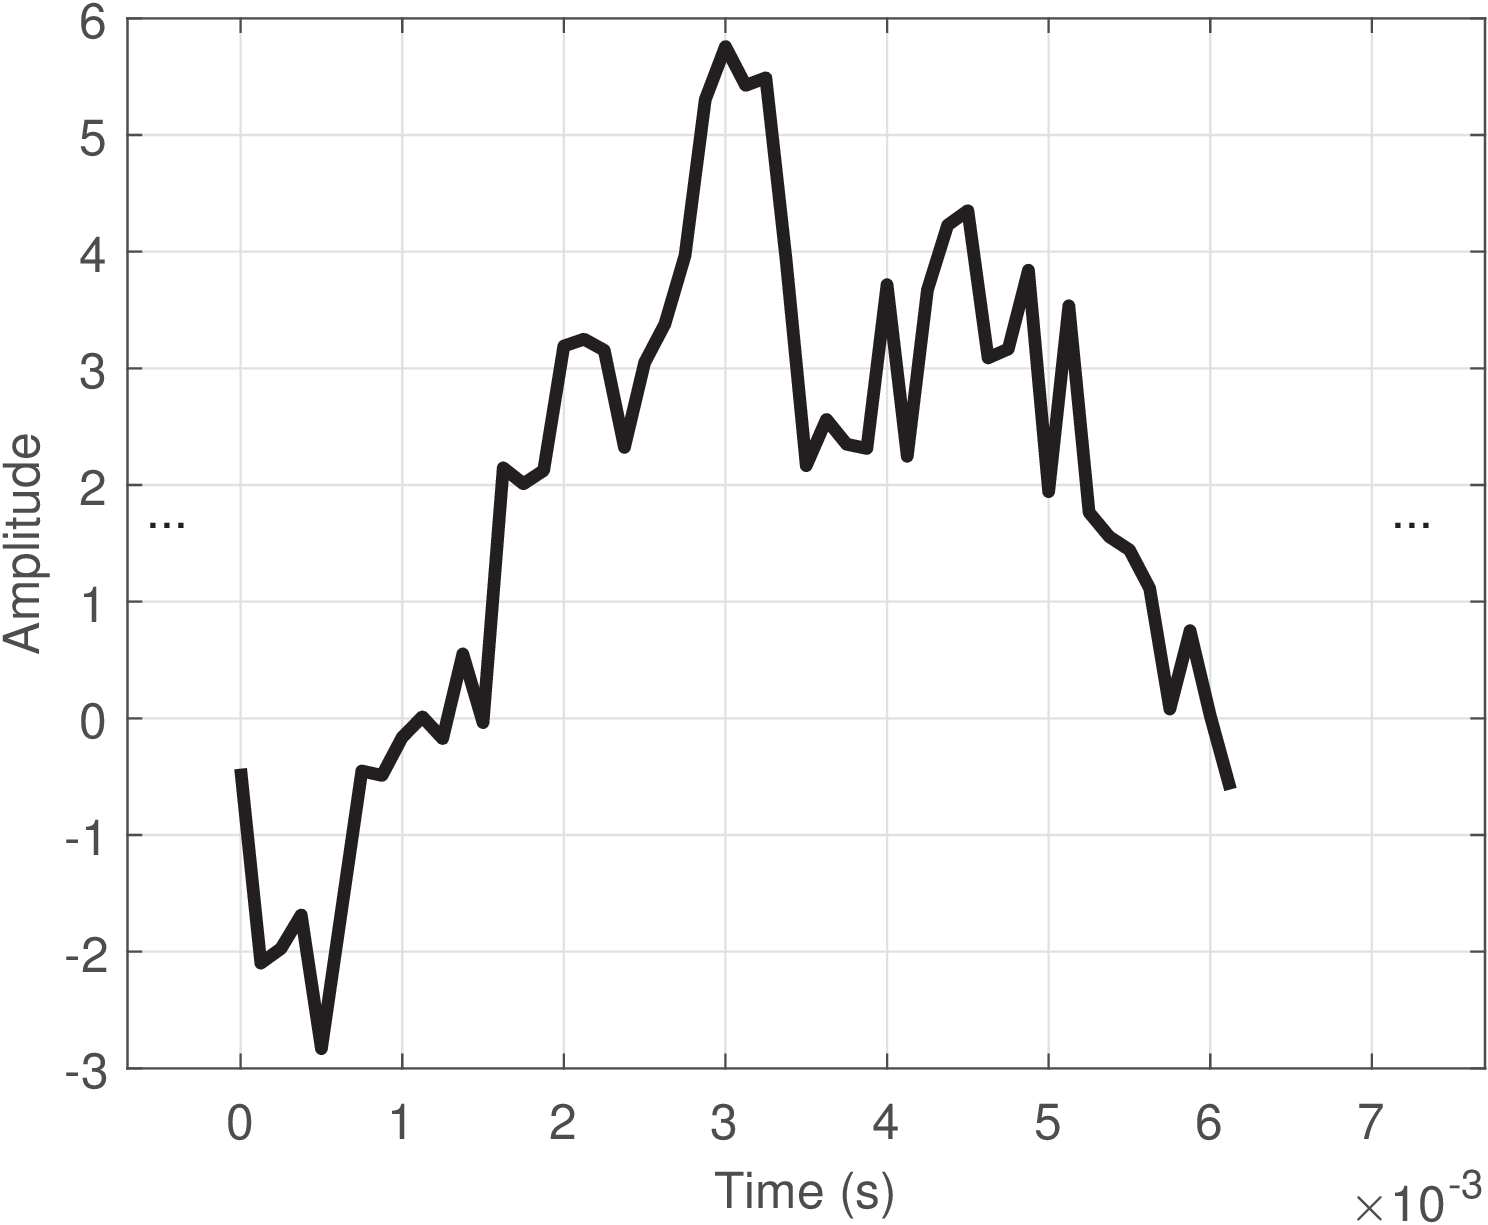
\includegraphics[width=\textwidth]{figures/analogsignal.png}
      \caption{Image 1}
    \end{subfigure}
    \begin{subfigure}{0.45\textwidth}
      \centering
      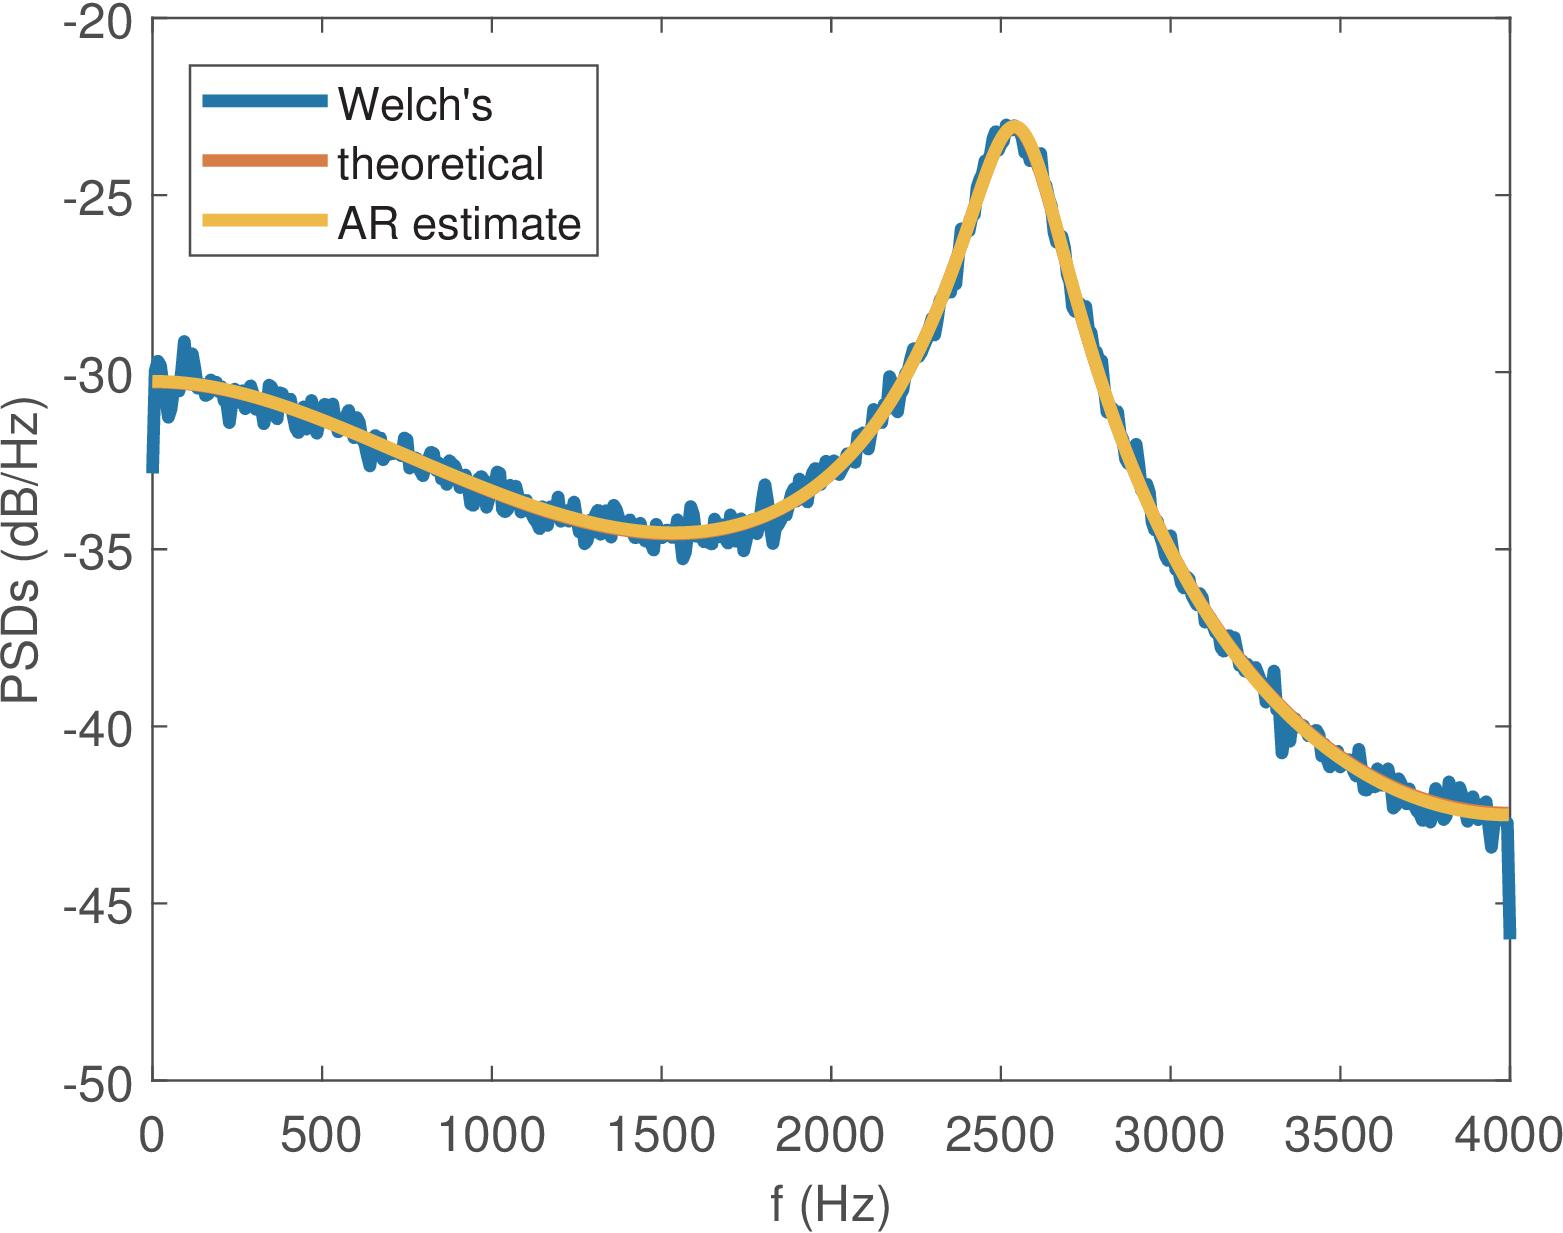
\includegraphics[width=\textwidth]{figures/arSpectrumMatched.png}
      \caption{Image 2}
    \end{subfigure}
    \caption{Main Caption}
  \end{figure}

\begin{equation}
    x(t) = \left\{ {\begin{array}{*{20}c} {A,~-T/2 \le t \le T/2} \\ {~ 0,{~\textrm{otherwise}}} \\ \end{array} \Leftrightarrow } \right. X(f) = A T sinc(fT)
    \label{eq:sinc_transform}
    \end{equation}


\[
x(t) \arrowedbox{SAMPLING} x_s(t) \arrowedbox{S/D} x[n] \arrowedbox{{$\tilde{Q}_c$}} x_b[n],
\]

\[
x(t) \arrowedbox{SAMPLING} x_s(t) \arrowedbox{S/D} x[n] \rightarrow\boxed{\tilde{Q}_c}\rightarrow x_b[n],
\]

$\fbox{$\sin(x)$}$



\begin{align*}
    \left[
    \begin{array}{l}
            x(0) \\ x(1) \\ x(2) \\ x(3)
    \\ \end{array}
    \right]
    &=
    \frac{1}{2}
    \left[ \begin{array}{cccc}
     1 &  1.307 & 1 & 0.541 \\
     1 &  0.541 & -1 & -1.307 \\
     1 &  -0.541 & -1 & 1.307 \\
     1 &  -1.307 & 1 & -0.541 \\ \end{array} \right]
    \left[
    \begin{array}{c}
            5 \\ -2.230 \\ 0 \\ -0.158
    \\ \end{array}
    \right]
    \\
    &=
    \frac{1}{2} \left\{
    5
    \left[
    \begin{array}{c}
            1 \\ 1 \\ 1 \\ 1
    \\ \end{array}
    \right]
    - 2.230
    \left[
    \begin{array}{c}
            1.307 \\ 0.541 \\ -0.541  \\ -1.307
    \\ \end{array}
    \right] \right.\\
    &\mathrel{\ifpdf \phantom{=} \else \fbox{\phantom{=}} \fi} \left. +0
    \left[
    \begin{array}{c}
            1 \\ -1 \\ -1 \\ 1
    \\ \end{array}
    \right]
    -0.158
    \left[
    \begin{array}{c}
            0.541 \\ -1.307 \\ 1.307 \\ -0.541
    \\ \end{array}
    \right]
    \right\}.
    \end{align*}



\begin{align*}
    \left[
    \begin{array}{l}
            x(0) \\ x(1) \\ x(2) \\ x(3)
    \\ \end{array}
    \right]
    &=
    \frac{1}{2}
    \left[ \begin{array}{cccc}
     1 &  1.307 & 1 & 0.541 \\
     1 &  0.541 & -1 & -1.307 \\
     1 &  -0.541 & -1 & 1.307 \\
     1 &  -1.307 & 1 & -0.541 \\ \end{array} \right]
    \left[
    \begin{array}{c}
            5 \\ -2.230 \\ 0 \\ -0.158
    \\ \end{array}
    \right]
    \\
    &=
    \frac{1}{2} \left\{
    5
    \left[
    \begin{array}{c}
            1 \\ 1 \\ 1 \\ 1
    \\ \end{array}
    \right]
    - 2.230
    \left[
    \begin{array}{c}
            1.307 \\ 0.541 \\ -0.541  \\ -1.307
    \\ \end{array}
    \right] \right.\\
    &\mathrel{\phantom{=}} \left. +0    \left[
    \begin{array}{c}
            1 \\ -1 \\ -1 \\ 1
    \\ \end{array}
    \right]
    -0.158
    \left[
    \begin{array}{c}
            0.541 \\ -1.307 \\ 1.307 \\ -0.541
    \\ \end{array}
    \right]
    \right\}.
\end{align*}

\end{document}